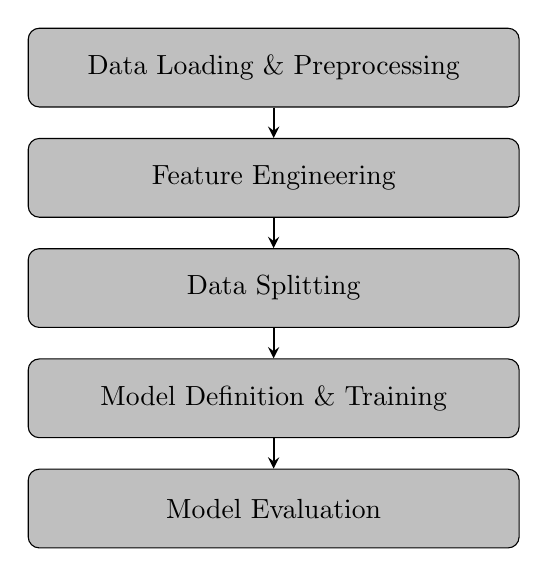
\begin{tikzpicture}[scale=0.7]
    % Define the styles for the processes and arrows
    \tikzstyle{process}=[rectangle, rounded corners, draw=black, fill=lightgray, text centered, text width=6cm, minimum height=1cm]
    \tikzstyle{arrow}=[thick,->,>=stealth]

    % Draw the processes
    \node[process] (data_loading) at (0, 0) {Data Loading \& Preprocessing};
    \node[process] (feature_engineering) at (0, -2) {Feature Engineering};
    \node[process] (data_splitting) at (0, -4) {Data Splitting};
    \node[process] (model_definition) at (0, -6) {Model Definition \& Training};
    \node[process] (model_evaluation) at (0, -8) {Model Evaluation};

    % Draw the arrows between the processes
    \draw[arrow] (data_loading) -- (feature_engineering);
    \draw[arrow] (feature_engineering) -- (data_splitting);
    \draw[arrow] (data_splitting) -- (model_definition);
    \draw[arrow] (model_definition) -- (model_evaluation);
\end{tikzpicture}
